% Provenance (never printed): old premiere S material on plate kinematics (rigid
% plates, rates from magnetic anomalies and from satellite positioning, hotspots
% and the Hawaiian chain, the coherence of the model); see
% sources/book2/PROVENANCE.md. Velocities from the NNR-MORVEL56 poles
% (figdata/grade-11/plate_velocities.py), station series from the Nevada Geodetic
% Laboratory (gnss_series.py), volcano ages from Clague and Dalrymple 1987
% (hawaii_chain.py). Euler poles and triple junctions belong to Year 1: the
% rotation pole is told, not defined.
\chapter{板块及其运动}\label{ch:g11:plate-motions}

在夏威夷岛上的莫纳克亚山顶附近，一台固定在
岩石上的天线，自
1996 年 10 月起，每天都在接收定位卫星的信号。计算机每天算出天线的位置，
精确到几毫米。三十年的位置记录每年都讲述同一个故事：
天线、山体以及整个海岛，以每年约 \qty{7}{cm} 的速度
向西北偏西方向运动，不停歇，也不转向。到 2026 年，
天线已离开出发点两米多。本章测量这类运动，
说明它们如何在球面上相互配合，
并在从夏威夷延伸、横穿北太平洋的一串死火山链中，
读出同一种运动。
% ledger: data:b2-ngl-gnss

\begin{recall}
\omterm{def:g11:lithosphere-asthenosphere:lithosphere}{岩石圈}被分割成若干构造板块，它们彼此\omterm{def:g11:plate-motions:relative-motion}{相对运动}，
速率约为每年几厘米；板块的边界包括洋中脊、海沟、
碰撞带和转换断层（第 1 册，七年级）。热点是地幔深处的一个位置，
为其上方板块上的火山提供岩浆；板块
带着火山远离，新火山则在热点上方形成（第 1 册，
七年级）。卫星定位接收机利用几颗卫星的信号，
算出自身位置（第 1 册，九年级）。洋底的磁条带
给出洋中脊的扩张速率
（见\cref{ch:g11:drift-to-spreading}），\omterm{def:g11:lithosphere-asthenosphere:lithosphere}{岩石圈}是地球坚硬的外壳，
厚约 \qty{100}{km}
（见\cref{ch:g11:lithosphere-asthenosphere}）。速率为每年 \qty{1}{cm}，
即每百万年 \qty{10}{km}；每年 \qty{1}{mm}，
即每百万年 \qty{1}{km}。
\end{recall}

\begin{omfigure}
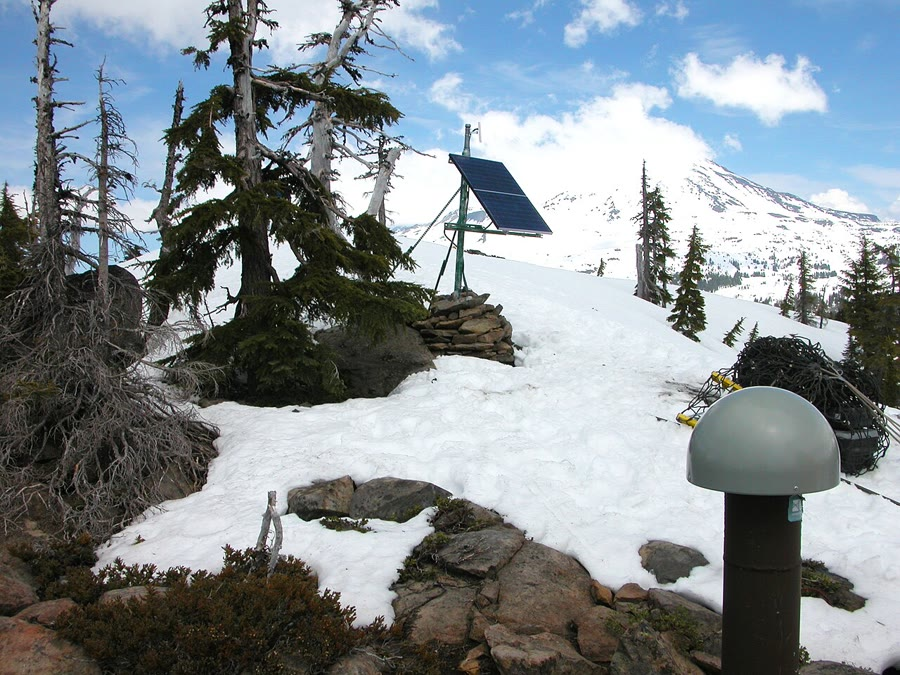
\includegraphics[width=0.62\linewidth]{images/book2/g11-usgs-gps-station.jpg}

{\small 美国俄勒冈州喀斯喀特山脉一座火山上的永久性卫星定位站（2007 年）。
天线位于灰色圆顶之下，装在立杆上，
立杆牢牢埋入地面；后方的太阳能板为接收机供电。这类站点
每天记录自身位置。照片：Dave Sherrod,
USGS（公有领域）。}
\end{omfigure}
% ledger: photo:g11-gps-station

\section{球面上的刚性板块}

地震并非随机分布于地球表面：绝大多数地震
发生在狭窄的带状地带，即板块边界（第 1 册，七年级）。板块
内部的岩石几乎完全不断裂。因此，板块并非随运动而拉伸、皱缩的软皮，
而是一块坚硬的\omterm{def:g11:lithosphere-asthenosphere:lithosphere}{岩石圈}，
整体一起运动。

\begin{definition}[刚性板块]\label{def:g11:plate-motions:rigid-plate}
称\emph{刚性板块}\index{刚性板块}为一块\omterm{def:g11:lithosphere-asthenosphere:lithosphere}{岩石圈}，它
作为单一块体运动：其上两点间的距离不变，
其形变集中于沿边界的狭窄带中。
\end{definition}

\omterm{def:g11:plate-motions:rigid-plate}{刚性板块}模型只是一种近似。某些地区的形变可延伸数百
千米，例如喜马拉雅山背后的高原以及北美西部，
模型把它们视为较宽的边界。但在地球表面的大部分区域，
该模型的效果相当好：其预测的\omterm{def:g11:plate-motions:rigid-plate}{刚性板块}速度
与卫星站实测值相符，误差在每年几毫米以内，
（见\cref{sec:g11:plate-motions:predictive}），而板块彼此之间的\omterm{def:g11:plate-motions:relative-motion}{相对运动}
速率为每年几厘米。

\omterm{def:g11:plate-motions:rigid-plate}{刚性板块}怎样在球面上运动？它不能沿直线滑动，
因为直线会离开球面。无论\omterm{def:g11:plate-motions:rigid-plate}{刚性板块}如何运动，
它都是绕过地心的某一轴线的\emph{旋转}。
该轴与地表相交于板块的\emph{旋转极}。板块上的一点
沿绕该极的小圆运动，离极越远，
小圆越大，运动越快
（见下图）。证明\omterm{def:g11:plate-motions:rigid-plate}{刚性板块}的任何运动都是这种旋转，
以及用旋转极描述板块边界，
属于第 3 册；本节只用到速率。

\begin{omfigure}
\begin{tikzpicture}[scale=1.15, font=\footnotesize]
  \fill[omSea!45] (0,0) circle (2);
  \draw (0,0) circle (2);
  % small circles about the rotation pole (pole at the top), seen slightly from above
  \foreach \a/\len in {60/0.75, 35/1.23, 0/1.5} {
    \pgfmathsetmacro{\r}{2*cos(\a)}
    \pgfmathsetmacro{\h}{2*sin(\a)}
    \draw[black!45, densely dashed] (-\r,\h) arc[start angle=180, end angle=0, x radius=\r, y radius=0.22*\r];
    \draw[omDef!80!black, line width=0.7pt] (-\r,\h) arc[start angle=180, end angle=360, x radius=\r, y radius=0.22*\r];
    \draw[-{Stealth[length=5pt]}, omProp, line width=1.1pt] (0,\h-0.22*\r) -- ++(\len,0);
  }
  \draw[black!70, dash pattern=on 3pt off 2pt] (0,-2.5) -- (0,2.55);
  \fill (0,2) circle (1.6pt);
  \node[anchor=south west] at (0.05,2.02) {旋转极};
  \node[anchor=north, text=black!70] at (0,-2.5) {通过地心的旋转轴};
  \fill (0,0) circle (1pt);
  \node[anchor=west, align=left] at (2.25,0.9) {各点运动 \\沿小圆 \\绕极};
  \node[anchor=west, align=left, text=omProp] at (2.25,-0.4) {速率在离极 \\\ang{90}处最大};
\end{tikzpicture}

{\small 球面上的\omterm{def:g11:plate-motions:rigid-plate}{刚性板块}绕通过地心的轴转动。
靠近旋转极的点沿小圆缓慢运动；
离极 \ang{90} 的点运动最快（箭头按比例表示速率）。}
\end{omfigure}

点的速率很容易算出。设某点与旋转极的角距离为
$\theta$，则它到轴的距离为 $R\sin\theta$，其中
$R = \qty{6371}{km}$ 为地球半径。若板块每百万年转过 $\omega$
度，则该点每百万年走过所在圆周的 $\omega/360$，
即圆周半径为 $R\sin\theta$：
\[
  v = \frac{\omega}{360} \times 2\pi R\sin\theta
    = \frac{\pi\,\omega}{180}\,R\sin\theta .
\]
当 $\omega = \qty{1}{\degree}$（每百万年）且 $\theta = \ang{90}$ 时，
速率约为 $\pi \times 6371/180 \approx \qty{111}{km}$ 每百万年，
即每年 \qty{11.1}{cm}。因此板块没有单一的速率：其上各点的速率
从旋转极处（若极位于板块上）的零
变化到离极 \ang{90} 处的最大值。洋中脊上使两板块相互错动的转换断层，
沿绕两板块相对旋转
极的小圆延伸。
% ledger: earth:Rmean (shared), nnr56:poles

已发布的转动极数据给出每个板块的极位置及其转动速率。其中一套
主要由沿洋脊测得的扩张速率和扩张方向构建，
描述了 56 个板块；太平洋板块的
转动速率为
每百万年 \ang{0.651}，欧亚板块为 \ang{0.223}。由这些数值，
计算机即可求得任一板块上任一点的速度
（见下图）。
% ledger: nnr56:poles, nnr56:data

\begin{omfigure}
\begin{tikzpicture}
\begin{axis}[ommap, width=\linewidth, xtick={-180,-90,...,180}, ytick={-60,0,60}]
\addplot[fill=omLithAlluv, draw=black!45, line width=0.2pt] table {figdata/out/shared-geo-land.dat};
\addplot[omRidge, line width=0.6pt] table {figdata/out/shared-geo-school-ridge.dat};
\addplot[omRidge!70!black, line width=0.6pt] table {figdata/out/shared-geo-school-transform.dat};
\addplot[omTrench, line width=0.6pt] table {figdata/out/shared-geo-school-subduction.dat};
\addplot[fill=omTrench, draw=none] table {figdata/out/shared-geo-school-teeth.dat};
\addplot[black!65, line width=0.6pt] table {figdata/out/shared-geo-school-collision.dat};
% computed in figdata/grade-11/plate_velocities.py (NNR-MORVEL56); 2.5 degrees per cm/yr
\addplot[black, line width=0.8pt, -{Stealth[length=4pt]}, quiver={u=\thisrow{dx}, v=\thisrow{dy}}]
  table[x=lon, y=lat] {figdata/out/grade-11-plate_velocities-arrows.dat};
\addplot[omProp, line width=1.2pt, -{Stealth[length=5pt]}, quiver={u=\thisrow{dx}, v=\thisrow{dy}}]
  table[x=lon, y=lat] {figdata/out/grade-11-plate_velocities-hawaii.dat};
\addplot[only marks, mark=*, mark size=1.3pt, omProp] coordinates {(-155.46,19.80)};
\node[font=\scriptsize, anchor=north, fill=white, fill opacity=0.75, text opacity=1, inner sep=1pt]
  at (axis cs:-150,15) {莫纳克亚山};
\draw[black, line width=0.8pt, -{Stealth[length=4pt]}] (axis cs:-172,-80) -- (axis cs:-147,-80);
\node[font=\scriptsize, anchor=west, fill=white, fill opacity=0.75, text opacity=1, inner sep=1pt]
  at (axis cs:-145,-80) {\qty{10}{cm} 每年};
\end{axis}
\end{tikzpicture}

{\small 图中为 16 个板块内各点的速度，由已发布的转动极算得，
参考系中整个\omterm{def:g11:lithosphere-asthenosphere:lithosphere}{岩石圈}整体不转动。
太平洋、纳斯卡、科科斯、澳大利亚和印度板块运动最快；
欧亚、北美、南美和南极板块运动较慢。红色箭头：
莫纳克亚山处的太平洋板块。转动极数据：Argus、Gordon 和 DeMets
（2011）；板块边界：Bird（2003）；陆地：Natural Earth。}
\end{omfigure}
% ledger: nnr56:poles, data:pb2002, data:ne-land

\section{测量运动}

\subsection{测量速度的两种方法}

海底的磁条带给出两个板块跨越洋脊相互远离的速度
（见\cref{ch:g11:drift-to-spreading}）：用条带到洋脊轴线的距离除以其年龄。
所得速度是条带年龄上的平均，通常对应最近几百万年，
并且它是\emph{相对}速度，即一个板块相对另一个板块的速度。磁条带
无法说明在海沟或碰撞带相遇的板块，
因为那里
不生成洋底。

卫星定位测量的是单个点当前的运动，
时间跨度为几年或几十年。永久观测站固定在坚硬的基岩上，
从而随板块运动；其每日位置对时间作图后，
沿一条直线排列，该直线的斜率即为测站的速度。

\begin{method}[由定位时间序列求速率]\label{met:g11:plate-motions:rate}
\begin{enumerate}
  \item 将测站的东向与北向位置对时间作图，
        可画在两幅图上，也可画在同一幅图上。
  \item 画出最贴合每组数据的直线（或在其上读取相距较远的两点），
        其斜率（以毫米每年计）即为东向速度 $v_E$ 或北向速度 $v_N$；
        向西或向南运动的测站，
        其速度为负值。
  \item 测站的速度为 $v = \sqrt{v_E^2 + v_N^2}$；其方向
        与东–西向直线的夹角 $\alpha$ 满足
        $\tan\alpha = |v_N|/|v_E|$，若 $v_N > 0$ 则偏北，
        若 $v_E > 0$ 则偏东。
\end{enumerate}
\end{method}

\begin{omfigure}
\begin{tikzpicture}
\begin{axis}[ompt, name=a, width=0.5\linewidth, height=5.6cm, xmin=1995, xmax=2027, ymin=-200, ymax=120,
  xlabel={年}, ylabel={位置（\unit{cm}）}, xtick={2000,2010,2020},
  xticklabel style={/pgf/number format/set thousands separator={}},
  title={\small 莫纳克亚山，夏威夷（MKEA）}, tick label style={font=\scriptsize}]
% computed in figdata/grade-11/gnss_series.py; ledger: data:b2-ngl-gnss
\addplot[only marks, mark=*, mark size=0.5pt, omDef] table[x=year, y=north] {figdata/out/grade-11-gnss_series-mkea.dat};
\addplot[only marks, mark=*, mark size=0.5pt, omProp] table[x=year, y=east] {figdata/out/grade-11-gnss_series-mkea.dat};
\node[font=\scriptsize, text=omDef!80!black, anchor=west] at (axis cs:1996.5,80) {北向};
\node[font=\scriptsize, text=omProp!80!black, anchor=west] at (axis cs:1996.5,-120) {东向};
\end{axis}
\begin{axis}[ompt, at={(a.east)}, anchor=west, xshift=0.9cm, width=0.5\linewidth, height=5.6cm, xmin=1995, xmax=2027,
  ymin=-10, ymax=70, xlabel={年}, xtick={2000,2010,2020},
  xticklabel style={/pgf/number format/set thousands separator={}},
  title={\small 韦策尔，德国（WTZR）}, tick label style={font=\scriptsize}]
\addplot[only marks, mark=*, mark size=0.5pt, omDef] table[x=year, y=north] {figdata/out/grade-11-gnss_series-wtzr.dat};
\addplot[only marks, mark=*, mark size=0.5pt, omProp] table[x=year, y=east] {figdata/out/grade-11-gnss_series-wtzr.dat};
\node[font=\scriptsize, text=omDef!80!black, anchor=west] at (axis cs:2014,22) {北向};
\node[font=\scriptsize, text=omProp!80!black, anchor=west] at (axis cs:2006,40) {东向};
\end{axis}
\end{tikzpicture}

{\small 两个永久观测站从第一个月起的月平均位置：东向（红色）和北向（蓝色）。
每组数据都沿一条直线排列，该直线的斜率即为测站在该方向上的速度。
莫纳克亚山位于太平洋板块上，向西、向北运动；
韦策尔位于欧亚板块上，向东、向北运动，速度约慢三倍。数据来源：
Nevada Geodetic Laboratory（Blewitt、哈蒙德和 Kreemer，2018）。}
\end{omfigure}
% ledger: data:b2-ngl-gnss

\begin{example}[莫纳克亚山上的测站]\label{ex:g11:plate-motions:mkea}
从 1996 年 10 月到 2026 年 9 月，莫纳克亚山测站的月位置
沿两条直线变化，斜率为 $v_E =
\qty{-63.2}{mm}$ 每年（向西），$v_N = \qty{+34.5}{mm}$ 每年。
速度为 $\sqrt{63.2^2 + 34.5^2} \approx \qty{72}{mm}$ 每年，又由 $\tan\alpha
= 34.5/63.2 \approx 0.546$ 得 $\alpha \approx \ang{29}$：测站
以 \qty{7.2}{cm} 每年的速度，沿西偏北 \ang{29} 的方向运动。太平洋板块的转动极
预测此处的运动为 \qty{6.9}{cm} 每年，
方向为西偏北 \ang{28}。
\end{example}
% ledger: data:b2-ngl-gnss, nnr56:poles (prediction computed in plate_velocities.py)

各点围绕直线散布仅几毫米，远小于单年的运动量：
经过几年测量，测站速度的精度可优于
每年 1 毫米。

\subsection{相对运动与绝对运动}

速度总是相对于某个参照系而言的。莫纳克亚山测站
相对于与整个地球固连的参照系，以 \qty{7.2}{cm} 每年的速度运动；
而从北美的一个测站看去，由于该测站本身也在运动，
其速度则不同。

\begin{definition}[相对运动；绝对运动]\label{def:g11:plate-motions:relative-motion}
\emph{相对运动}\index{相对运动}是板块 $A$ 相对于板块 $B$ 的运动，
即站在 $B$ 上的观察者所看到的运动。
\emph{绝对运动}\index{绝对运动}是板块相对于与深部地球固连的
参照系的运动，参照系可取为一组假定固定的热点，
或\omterm{def:g11:lithosphere-asthenosphere:lithosphere}{岩石圈}整体不发生转动的
参照系。
\end{definition}

脊、海沟和转换断层的形态由\omterm{def:g11:plate-motions:relative-motion}{相对运动}决定：
边界处关心的是两块板块彼此之间如何运动。
相对速度与它们所产生的位移一样，可以相加。

\begin{proposition}[相对速度如矢量般相加]\label{prop:g11:plate-motions:sum}
设 $\vec v_{A/B}$ 为板块 $A$ 相对于板块 $B$ 的速度，
取边界上给定的一点，其他各对板块同理。对任意
三块板块 $A$、$B$、$C$，
\[
  \vec v_{A/C} = \vec v_{A/B} + \vec v_{B/C},
  \qquad\text{和}\qquad
  \vec v_{B/A} = -\vec v_{A/B}.
\]
\end{proposition}

\begin{proof}
在很短的时间 $\Delta t$ 内，设与 $A$ 固连的一点自位置 $P$ 运动到
到 $P'$（自 $C$ 处看），又设 $B$ 上原在 $P$ 处的点运动到
$Q$（自 $C$ 处看）。自 $B$ 看，$A$ 上的该点已由 $Q$ 运动到
$P'$。位移按矢量相加：
$\overrightarrow{PP'} = \overrightarrow{PQ} + \overrightarrow{QP'}$，即
$A$ 的位移（自 $C$ 看）= $B$ 的位移（自 $C$ 看）+
$A$ 的位移（自 $B$ 看）。两边除以 $\Delta t$，得 $\vec v_{A/C}
= \vec v_{B/C} + \vec v_{A/B}$。取 $C = A$，左边为零，于是 $\vec
v_{B/A} = -\vec v_{A/B}$。
\end{proof}

\begin{method}[闭合速度三角形]\label{met:g11:plate-motions:triangle}
\begin{enumerate}
  \item 将每个已知速度按东、北两个分量写出，
        且均在同一点测量。
  \item 求 $\vec v_{A/B}$，已知 $A$、$B$ 在同一
        参照系 $C$ 中的速度，则相减：$\vec v_{A/B} = \vec v_{A/C} - \vec v_{B/C}$，
        逐分量计算。
  \item 在图上，将 $\vec v_{A/C}$ 与 $\vec v_{B/C}$ 的起点
        置于同一点：由 $\vec v_{B/C}$ 的终点指向
        $\vec v_{A/C}$ 的终点的箭头即为 $\vec v_{A/B}$，它闭合了三角形。
  \item 按
        \cref{met:g11:plate-motions:rate}计算其长度与方向。
\end{enumerate}
\end{method}

\begin{example}[圣安德烈亚斯断层]\label{ex:g11:plate-motions:san-andreas}
在加利福尼亚中部，北纬 \ang{35.5}、西经 \ang{120.5} 处，转动极给出
太平洋板块的速度为 $(-42.1, +26.4)$，北美板块为 $(-11.9, -14.8)$，
单位为毫米每年（东、北分量），参照系为整个\omterm{def:g11:lithosphere-asthenosphere:lithosphere}{岩石圈}。太平洋板块
相对于北美的运动为 $(-42.1 + 11.9,\ 26.4 + 14.8) = (-30.2, +41.2)$，即
$\sqrt{30.2^2 + 41.2^2} \approx \qty{51}{mm}$ 每年，
方向为西偏北 \ang{36}（见下图）。
圣安德烈亚斯断层走向西北，
承担了此运动的大部分滑动。
\end{example}
% ledger: nnr56:poles (computed in plate_velocities.py: relative pa/na at 120.5 W 35.5 N)

\begin{omfigure}
\begin{tikzpicture}[x=0.065cm, y=0.065cm, font=\footnotesize]
  % mm/yr, from plate_velocities.py: PA (-42.1, 26.4), NA (-11.9, -14.8), PA/NA (-30.2, 41.2)
  \draw[black!25] (-8,0) -- (8,0) (0,-8) -- (0,8);
  \draw[-{Stealth[length=5pt]}, omProp, line width=1.1pt] (0,0) -- (-42.1,26.4)
    node[pos=0.55, above right, inner sep=1pt] {$\vec v_{\mathrm{PA}}$};
  \draw[-{Stealth[length=5pt]}, omDef, line width=1.1pt] (0,0) -- (-11.9,-14.8)
    node[pos=0.8, right=2pt] {$\vec v_{\mathrm{NA}}$};
  \draw[-{Stealth[length=5pt]}, black, line width=1.1pt] (-11.9,-14.8) -- (-42.1,26.4)
    node[pos=0.4, left=9pt, align=right] {$\vec v_{\mathrm{PA/NA}}$\\\qty{51}{mm} 每年};
  \fill (0,0) circle (0.9pt);
  % compass
  \draw[-{Stealth[length=4pt]}] (25,10) -- (25,24) node[above] {北};
  \draw[-{Stealth[length=4pt]}] (25,10) -- (39,10) node[right] {东};
  \draw (25,-18) -- (40.4,-18);
  \node[below] at (32.7,-18) {\qty{20}{mm} 每年};
  \draw (25,-17) -- (25,-19) (40.4,-17) -- (40.4,-19);
\end{tikzpicture}

{\small 加利福尼亚中部速度三角形的闭合（按比例绘制）。红色：
太平洋板块；蓝色：北美板块，均在整个\omterm{def:g11:lithosphere-asthenosphere:lithosphere}{岩石圈}参照系中。
黑色：自北美看太平洋板块，
箭头由蓝色箭头的终点指向红色箭头的终点。}
\end{omfigure}

\section{热点轨迹}

\subsection{板块越过固定的地幔柱}

夏威夷位于太平洋板块的中部，
距最近的板块边界超过 \qty{3000}{km}。
% ledger: usgs:hawaii-hotspot (Book 1 row)
 其火山由一个热点供给（见第 1 册，
七年级）。板块在其上方运动，每座火山都被带离热点，
而新的火山则在其后方生成。

\begin{definition}[热点轨迹]\label{def:g11:plate-motions:hotspot-track}
称\emph{热点轨迹}\index{热点轨迹}为由火山及被称为海山的沉没火山
所构成的线状分布，这些火山在板块越过热点时被带离热点；
正在活动的火山位于热点上方，
离热点越远的火山年代越老。
\end{definition}

\begin{omfigure}
\begin{tikzpicture}[font=\footnotesize]
  % plate moving to the left over a fixed plume (not to scale)
  \fill[omSea!50] (0,0) rectangle (11,0.9);
  \fill[black!22] (0,-0.9) rectangle (11,0);
  \draw (0,0) -- (11,0);
  \draw[densely dashed] (0,0.9) -- (11,0.9) node[right] {海平面};
  \node[anchor=east] at (10.95,-0.45) {岩石圈};
  \fill[omLithPeridotite!40] (0,-2.3) rectangle (11,-0.9);
  \node[anchor=west] at (0.1,-1.6) {软流圈};
  % plume
  \fill[omProp!55] (8.6,-2.3) -- (8.6,-1.2) .. controls (8.6,-0.9) and (9.2,-0.9) .. (9.2,-1.2) -- (9.2,-2.3) -- cycle;
  \fill[omProp!55] (8.75,-0.95) rectangle (9.05,0);
  \node[anchor=north, align=center] at (8.9,-2.35) {地幔柱，固定于地幔中};
  % volcanoes: active over the plume, older ones carried left, eroded and sunk
  \fill[black!65] (8.0,0) -- (8.9,1.6) -- (9.8,0) -- cycle;
  \fill[black!55] (5.4,0) -- (6.2,1.15) -- (7.0,0) -- cycle;
  \fill[black!50] (3.0,0) -- (3.55,0.62) -- (3.85,0.62) -- (4.4,0) -- cycle;
  \fill[black!45] (0.8,0) -- (1.25,0.42) -- (1.65,0.42) -- (2.1,0) -- cycle;
  \node[above] at (8.9,1.6) {活动火山};
  \node[above] at (6.2,1.15) {$t_1$};
  \node[above] at (3.7,0.62) {$t_2$};
  \node[above] at (1.45,0.42) {$t_3$};
  % plate motion
  \draw[-{Stealth[length=6pt]}, line width=1.2pt] (6.5,-0.45) -- (4.0,-0.45) node[left] {板块运动，速度 $v$};
  % distance d = v t
  \draw[{Stealth[length=4pt]}-{Stealth[length=4pt]}] (3.7,2.3) -- (8.9,2.3) node[midway, above] {$d_2 = v\,t_2$};
  \draw[black!50] (3.7,1.05) -- (3.7,2.4) (8.9,2.0) -- (8.9,2.4);
\end{tikzpicture}

{\small 板块以速度 $v$ 越过固定于地幔中的地幔柱（未按比例绘制）。
年龄为 $t$ 的火山形成于地幔柱上方，已被带离的距离为 $d = v\,t$；
较老的火山受到侵蚀并沉没于
海平面之下。}
\end{omfigure}

\begin{proposition}[由热点轨迹求速度]\label{prop:g11:plate-motions:hotspot}
若热点固定于深部地幔中，其上方的板块以恒定速度 $v$ 沿恒定方向运动，则
曾位于热点上方、距今时间为 $t$ 的火山，
现位于距活动火山的距离为
\[
  d = v\,t
\]
处，沿轨迹方向。火山年龄与距离的关系图中，各点落在一条过原点的直线上，
该直线的斜率为 $1/v$，
$v$ 即为板块的绝对速度。
\end{proposition}

\begin{proof}
火山形成于板块位于热点上方之时，此后便随板块一起运动。
在时间 $t$ 内，板块沿固定方向移动了
$v\,t$，因此该火山与当前位于热点上方的板块点
（即活动火山所在处）相距此距离。
由 $t = d/v$ 可知，这是一条斜率为 $1/v$ 的过原点直线。
速度是相对于热点、即相对于深部地幔测得的，
因此是绝对速度。
\end{proof}

\subsection{夏威夷–帝王海山链}

从夏威夷岛出发，一条由岛屿、礁石和海山组成的链状结构
向西偏北延伸约 \qty{3400}{km}，随后急转，向北延续为帝王海山，
其中苏伊科海山位于距基拉韦厄
\qty{4860}{km} 处，并一直延伸至堪察加半岛和阿留申群岛外的海沟
（见下图）。
% ledger: cd87:ages

\begin{omfigure}
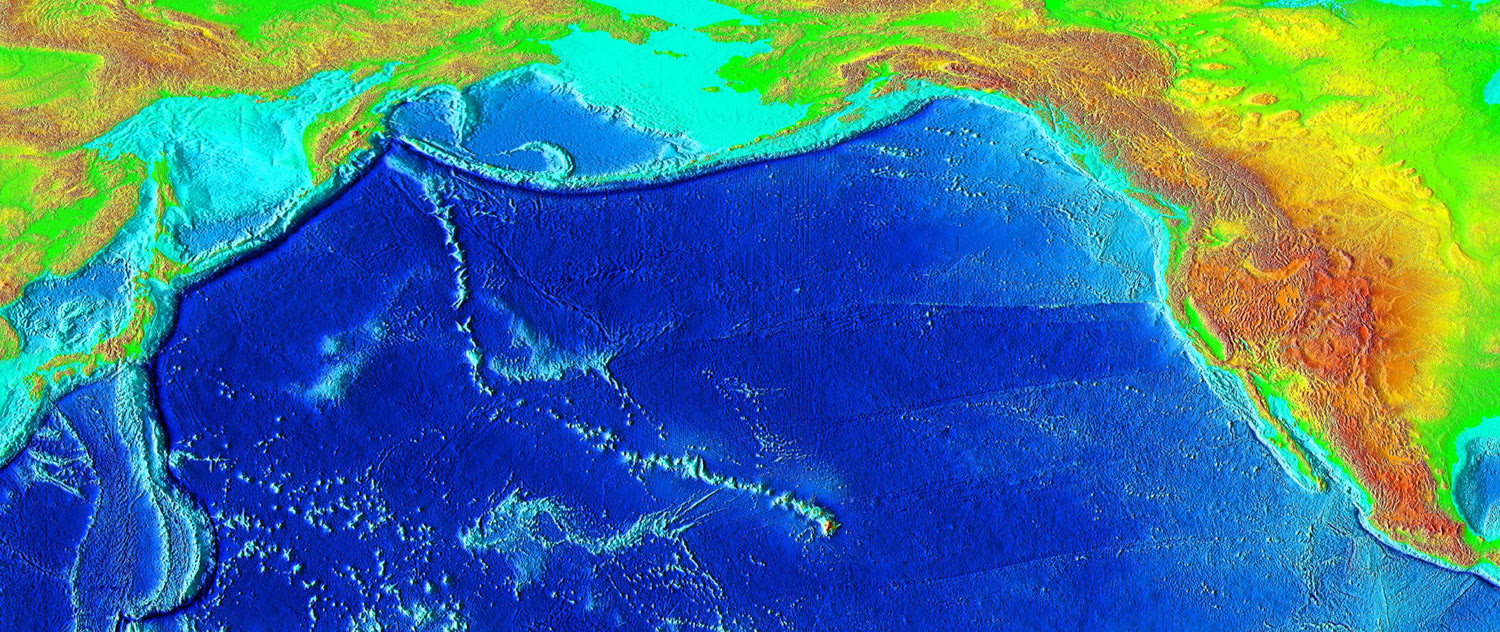
\includegraphics[width=\linewidth]{images/book2/g11-ngdc-hawaii-chain.jpg}

{\small 北太平洋海底的晕渲地形图。夏威夷链由夏威夷岛
（图下方中部，棕色）向西偏北延伸；在转折处转而向北，
形成帝王海山，最终止于沿堪察加半岛和阿留申群岛的海沟。
图像来源：美国国家海洋和大气管理局（NOAA）
国家地球物理数据中心（公有领域）。}
\end{omfigure}
% ledger: photo:g11-hawaii-chain

对链上 37 座火山的熔岩进行钾–氩测年，样品采自岛屿，
由海山拖网获取，或由其沉积物中钻取，
由此得到其年龄（见下图）。莫纳克亚火山约
40 万年，考艾岛为 \num{5.1}，中途岛为 \num{27.7}，
位于帝王海山链远端的苏伊科海山为 \num{64.7}。
年龄随距活动火山基拉韦厄的距离增大而增大，
与\omterm{def:g11:plate-motions:hotspot-track}{热点轨迹}的预测相符。
% ledger: cd87:ages

\begin{omfigure}
\begin{tikzpicture}
\begin{axis}[ompt, width=0.82\linewidth, height=6.4cm, xmin=0, xmax=5000, ymin=0, ymax=70,
  xlabel={沿链距基拉韦厄的距离（\unit{km}）}, ylabel={年龄（百万年）},
  xticklabel style={/pgf/number format/set thousands separator={}},
  legend style={font=\scriptsize, at={(0.03,0.97)}, anchor=north west}, legend cell align=left]
% computed in figdata/grade-11/hawaii_chain.py; ledger: cd87:ages
\addplot[only marks, mark=o, mark size=1.6pt, omDef, error bars/.cd, y dir=both, y explicit]
  table[x=dist, y=age, y error=err] {figdata/out/grade-11-hawaii_chain-hawaiian.dat};
\addplot[only marks, mark=triangle, mark size=2pt, omProp, error bars/.cd, y dir=both, y explicit]
  table[x=dist, y=age, y error=err] {figdata/out/grade-11-hawaii_chain-emperor.dat};
\addplot[black, densely dashed, line width=0.6pt] table[x=dist, y=age] {figdata/out/grade-11-hawaii_chain-fit.dat};
\legend{夏威夷链，转折处与帝王海山链，{过原点的直线，\qty{9.1}{cm} 每年}}
\draw[black!50, densely dotted] (axis cs:3400,0) -- (axis cs:3400,70);
\node[font=\scriptsize, anchor=south, rotate=90] at (axis cs:3400,8) {转折处};
\node[font=\scriptsize, anchor=north west] at (axis cs:519,5.1) {考艾岛};
\node[font=\scriptsize, anchor=south] at (axis cs:2432,30) {中途岛};
\node[font=\scriptsize, anchor=south east] at (axis cs:4860,65.5) {苏伊科};
\end{axis}
\end{tikzpicture}

={\small 夏威夷–帝王海山链火山的年龄与其到基拉韦厄火山的距离关系，
并标出年龄的不确定度。
沿夏威夷链，各点近似位于过原点的直线上；转折之后，年龄随距离增长得更快。
数据来源：Clague 和 Dalrymple
（1987）。}
\end{omfigure}

沿夏威夷链，在约 \qty{3300}{km} 以内，各点
围绕过原点的直线分布。最能拟合这一段 26 座已测龄火山的直线，
每隔 \qty{91}{km} 年龄增加一百万年：
由\cref{prop:g11:plate-motions:hotspot}可知，太平洋板块在热点上方的移动速率约为
每百万年 \qty{91}{km}，即每年 \qty{9.1}{cm}。
年龄数据的作者以自己的方式拟合整条链，
得到的速率为每年 \qty{8.6}{cm}。
% ledger: cd87:ages (fit computed in hawaii_chain.py), cd87:rate

转折之后，年龄随距离增长得更快：沿帝王海山链，
板块移动较慢，平均约为每年 \qty{6.5}{cm}
（由九座已测龄海山拟合的最佳直线）。链的走向也发生了改变。
若热点固定不动，转折处记录的便是太平洋板块运动方向的改变。
较新的年龄数据把转折的起点定在
钦明海山附近，约 5000 万年前，
这与太平洋扩张脊的重组以及
太平洋西缘岛弧最早火山的出现同时发生：
板块改变了方向。
% ledger: cd87:ages (Emperor fit computed in hawaii_chain.py), sc06:bend

\section{模型的预测能力}\label{sec:g11:plate-motions:predictive}

板块模型认为，少数\omterm{def:g11:plate-motions:rigid-plate}{刚性板块}绕各自的旋转极转动，
几乎所有的活动都发生在板块边界上。该模型的优势在于：
采用完全不同的方法、在时间跨度差异很大的
测量结果彼此一致。

\begin{itemize}
  \item \emph{地震与火山}集中分布在板块边界上，
        边界的类型决定了它们的类型：浅源地震见于洋中脊，
        深源地震只出现在海沟附近（\cref{ch:g11:subduction-zones}）。
  \item \emph{洋底}在洋中脊处最年轻，
        离洋中脊越远越老，两侧对称分布
        （\cref{ch:g11:drift-to-spreading}）。
  \item \emph{造山带}在板块汇聚处隆起：印度仍以
        每年约 \qty{4.5}{cm} 的速度朝欧亚板块推进，穿越喜马拉雅一带，
        这一数值由旋转极计算得出（\cref{ch:g12:mountain-building}）。
  \item \emph{各方法所得速度一致}：下表比较了今天由卫星定位测得的速度，
        与由旋转极预测的速度；后者的扩张速率主要来自磁条带，
        并对最近的运动取平均，
        取平均的时段为最近 \num{0.8} 至 320 万年，
        同时与\omterm{def:g11:plate-motions:hotspot-track}{热点轨迹}所记录的速度相比较，
        该速度跨越数千万年。
\end{itemize}
% ledger: nnr56:poles, nnr56:data (India-Eurasia computed in plate_velocities.py at 85 E 28 N)

\begin{center}
\small
\begin{tabular}{|l|c|c|}
\hline
测量对象 & 方法 & 速度（\unit{cm} 每年） \\ \hline
莫纳克亚，太平洋板块 & 卫星定位，30 年 & 7.2 \\
莫纳克亚，太平洋板块 & 旋转极 & 6.9 \\
韦策尔，欧亚板块 & 卫星定位，31 年 & 2.6 \\
韦策尔，欧亚板块 & 旋转极 & 2.3 \\
太平洋板块在夏威夷热点上方 & 火山年龄，4000 万年 & 9.1 \\ \hline
\end{tabular}
\end{center}
% ledger: data:b2-ngl-gnss, nnr56:poles, cd87:ages (all computed in figdata/grade-11)

旋转极给出的速度与台站测得的速度，相差不超过
每年 \qty{0.3}{cm}，尽管前者平均的是数百万年，后者仅有几十年：
板块今天的运动方式，与它们数百万年来的运动方式相同。
热点的速度较大：它是在另一参考系中测得的，
即热点自身的参考系，并且时间跨度也长得多。

比较整个板块的速度时，还能看出另一规律。运动最快的板块，
即科科斯板块、纳斯卡板块、太平洋板块、澳大利亚板块和菲律宾海板块，
它们都有一条长边在海沟处俯冲进入地幔，平均速度
约为每年 \qty{6.5}{cm}。没有这类边界的板块，
包括欧亚板块、北美板块、南美板块、非洲板块
和南极板块，平均速度约为每年 \qty{2.4}{cm}。关于驱动板块运动的这一线索，
在\cref{ch:g11:subduction-zones}中讨论。
% ledger: nnr56:rms (means computed in plate_velocities.py)

\section{练习}

\begin{exercise}[$\star$]\label{exo:g11:plate-motions:1}
给出\omterm{def:g11:plate-motions:rigid-plate}{刚性板块}的定义。\omterm{def:g11:lithosphere-asthenosphere:lithosphere}{岩石圈}的形变集中在何处，
哪一种日常可见的地震现象能说明这一点？
\end{exercise}

\begin{exercise}[$\star$]\label{exo:g11:plate-motions:2}
莫纳克亚台站每年移动 \qty{72}{mm}。将这一速率换算为
每百万年多少千米。台站在 30 年内移动了多远？
在一百万年内又移动了多远？
\end{exercise}

\begin{exercise}[$\star$]\label{exo:g11:plate-motions:3}
十年间，某台站向东移动了 \qty{30}{cm}，向北移动了 \qty{40}{cm}。求
其向东与向北的速度分量、速率，以及其运动方向与正北方向
所成的夹角。
\end{exercise}

\begin{exercise}[$\star$]\label{exo:g11:plate-motions:4}
给出\omterm{def:g11:plate-motions:hotspot-track}{热点轨迹}的定义。沿夏威夷链，最年轻的火山位于何处，
年龄沿哪个方向增大？这对太平洋板块的运动方向
说明了什么？
\end{exercise}

\begin{exercise}[$\star$]\label{exo:g11:plate-motions:5}
考艾岛沿该链位于距基拉韦厄火山 \qty{519}{km} 处，其最老的熔岩
年龄为 510 万年。假定热点固定不动，板块携带它
移动的平均速率是多少？请分别以每百万年千米数、
以及每年厘米数表示。
\end{exercise}

\begin{exercise}[$\star\star$]\label{exo:g11:plate-motions:6}
在两个测站序列的图中，韦策尔测站约
向东移动 \qty{63}{cm}、向北移动 \qty{48}{cm}，历时 31 年。
求其东向与北向速度、速度大小与方向，并与莫纳克亚
的速度作比较。
\end{exercise}

\begin{exercise}[$\star\star$]\label{exo:g11:plate-motions:7}
在冰岛，于北纬 \ang{64.5}、西经 \ang{18} 处，旋转极给出
北美板块的速度为 $(-10.5, +20.6)$，欧亚板块的速度为
$(+7.7, +16.3)$，单位为毫米每年（东向、北向）。(1) 求
北美板块相对欧亚板块的速度、速度大小与方向。(2) 穿过冰岛的洋中脊处该速度为多少？
(3) 将其与北大西洋常被引用的
\qty{2}{cm} 每年速率作比较。
\end{exercise}

\begin{exercise}[$\star\star$]\label{exo:g11:plate-motions:8}
太平洋板块每百万年转动 \ang{0.651}。(1) 求
距其旋转极 \ang{90} 处一点的速度（以厘米每年计）。(2) 求
距旋转极 \ang{30} 处一点的速度是多少？(3) 板块上何处速度为零？能否
用一个数表示整个板块的速度？
\end{exercise}

\begin{exercise}[$\star\star$]\label{exo:g11:plate-motions:9}
喜马拉雅山以北，于北纬 \ang{28}、东经 \ang{85} 处，旋转极
给出印度板块的速度为 $(+40.6, +38.6)$，欧亚板块的速度为
$(+24.0, -3.3)$，单位为毫米每年（东向、北向）。(1) 求印度相对欧亚的
速度、速度大小与方向。(2) 若运动保持
不变，则两板块在 1000 万年内将相互靠近多少？
\end{exercise}

\begin{exercise}[$\star\star$]\label{exo:g11:plate-motions:10}
内克尔距基拉韦厄 \qty{1058}{km}，年龄为 1030 万年；
中途岛距其 \qty{2432}{km}，年龄为 2770 万年。求
两座火山形成期间，板块在热点上方的速度。
并与 \qty{9.1}{cm} 每年作比较。
\end{exercise}

\begin{exercise}[$\star\star$]\label{exo:g11:plate-motions:11}
在某一点，板块 $A$ 相对板块 $B$ 以每年 \qty{3}{cm} 向东运动，
板块 $B$ 相对板块 $C$ 以每年 \qty{4}{cm} 向北运动。
(1) 画出速度三角形，求板块 $A$ 相对板块 $C$ 的速度：
大小与方向。(2) 求板块 $C$ 相对板块 $A$ 的速度。
\end{exercise}

\begin{exercise}[$\star\star\star$]\label{exo:g11:plate-motions:12}
莫纳克亚距基拉韦厄 \qty{54}{km}，年龄为 37.5 万
年。(1) 由此得出的板块速度是多少？(2) 火山直径为数十
千米，且生长持续数十万年。假设其到热点的距离
不确定 \qty{25}{km}，则速度位于哪个数值范围之间？
(3) 说明为何靠近热点的年轻火山
对速度的估计较差，而远离热点的火山
则更为可靠。
\end{exercise}

\begin{exercise}[$\star\star\star$]\label{exo:g11:plate-motions:13}
测站每月位置围绕其直线的散布约 \qty{5}{mm}，
运动量超过散布的十倍时，即可清楚地看出。
(1) 若要清楚看出莫纳克亚
测站每年 \qty{72}{mm} 的运动，需测量多久？(2) 若为每年 \qty{5}{mm} 的运动，
如大陆内部缓慢形变区域中所见，则需多久？(3) 为何板块速度
早在卫星能测量之前，
便已由磁条带测得？
\end{exercise}

\begin{exercise}[$\star\star\star$]\label{exo:g11:plate-motions:14}
在大西洋中脊南纬 \ang{30}、西经 \ang{13.5} 处，旋转
极给出南美板块的速度为 $(-4.9, +11.0)$，非洲板块的
速度为 $(+27.1, +17.9)$，单位为毫米每年（东向、北向）。
(1) 求南美板块相对非洲板块的速度、其大小与
方向。(2) 推算该洋脊的\omterm{def:g11:drift-to-spreading:spreading-rate}{全扩张速率}与半扩张速率。
(3) 南大西洋沉积物给出的半扩张速率约为 \qty{1.9}{cm}
每年，系过去 6600 万年的平均值
（见\cref{ch:g11:drift-to-spreading}）。比较二者，并推测
此差异可能意味着什么。
\end{exercise}

\begin{exercise}[$\star\star\star$]\label{exo:g11:plate-motions:15}
某测站稳定地每年向东移动 \qty{20}{mm}。恰在
十年观测的中点，一次地震使其突然移动 \qty{50}{mm}，
方向向西。(1) 画出其东向位置随时间变化的图像。(2) 仅由首末两点，
可求得多大的速度？(3) 数据序列的两半各自
能给出多大的速度？(4) \omterm{def:g10:measuring-the-earth:geodesy}{大地测量学}家应如何
处理这种跳跃？
\end{exercise}

\section{问题：解读夏威夷–帝王海山链}

\begin{problem}[{周末问题——板块速度写在火山之中}]
\label{pb:g11:plate-motions:1}
% values from Clague and Dalrymple 1987, Table 1.4 (ledger cd87:ages); fits computed in
% figdata/grade-11/hawaii_chain.py (v_hawaiian 91.2, v_emperor_free 64.6); bend sc06:bend;
% MKEA rates data:b2-ngl-gnss
表中给出了沿链测得的各火山与基拉韦厄火山的距离，以及
夏威夷–帝王海山链上十三座火山的钾–氩年龄。
基拉韦厄是位于热点之上的活火山；拐折位于阿博特
与大觉寺之间。

\begin{center}
\small
\begin{tabular}{|l|c|c||l|c|c|}
\hline
火山 & 距离（\unit{km}） & 年龄（\unit{Ma}） & 火山 & 距离（\unit{km}） & 年龄（\unit{Ma}） \\ \hline
莫纳克亚 & 54 & 0.375 & 阿博特 & 3280 & 38.7 \\ \hline
考艾岛 & 519 & 5.1 & 大觉寺 & 3493 & 42.4 \\ \hline
尼豪 & 780 & 7.2 & 高科（南） & 3758 & 48.1 \\ \hline
内克尔 & 1058 & 10.3 & 应神 & 4102 & 55.2 \\ \hline
莱桑 & 1818 & 19.9 & 仁德 & 4452 & 56.2 \\ \hline
中途岛 & 2432 & 27.7 & 推古（中） & 4860 & 64.7 \\ \hline
科拉汉 & 3128 & 38.6 & & & \\ \hline
\end{tabular}
\end{center}

\medskip
\noindent\textbf{第一部分——年龄与距离。}
\begin{enumerate}
  \item 表中哪座火山最年轻，哪座最古老？沿这条链，
        年龄如何变化？
  \item 证明：以千米计的距离除以以百万年计的年龄，
        所得即为以毫米每年计的速度。
  \item 计算由考艾岛给出的平均速率 $d/t$。
  \item 计算内克尔、莱桑、中途岛、科拉汉和阿博特的 $d/t$。
  \item 对表中位于弯折之前的八座火山，画出年龄关于距离的图。
        这些数据点是否接近
        一条过原点的直线？
\end{enumerate}

\medskip
\noindent\textbf{第二部分——板块相对热点的速度。}
\begin{enumerate}[resume]
  \item 解释为何当热点固定、板块以稳定的
        速度 $v$ 运动时，年龄 $t$ 与距离 $d$ 满足 $t = d/v$。
  \item 计算第~4~题中五个速度的平均值。
  \item 过原点且最佳拟合夏威夷链上全部 26 座有年代数据火山的直线，
        给出的速度为每百万年 \qty{91}{km}。
        与第~7~题比较。
  \item 以此速度，板块把考艾岛从热点处搬运至
        现在的位置需要多长时间？并与其年龄比较。
  \item 太平洋板块相对热点向哪个方向运动？
\end{enumerate}

\medskip
\noindent\textbf{第三部分——弯折处。}
\begin{enumerate}[resume]
  \item 计算板块在大觉寺火山与推古（中）火山
        形成的时刻之间的平均速率。
  \item 自大觉寺起的九座有年代数据的火山，其最佳拟合直线
        给出的速度为每百万年 \qty{65}{km}。与
        夏威夷链的速度相比较。
  \item 较新的年龄表明，弯折的起点位于钦明海山附近，
        距基拉韦厄 \qty{3668}{km}，约 5000 万年前。
        由此可得整条夏威夷链的平均速率为多少？
        与每百万年 \qty{91}{km} 作比较，并解释为何两者都
        可以成立。
  \item 若热点保持不动，弯折处记录了关于
        太平洋板块的什么信息？
  \item 较新的测年发现，沿天皇海山链的速度变化很大，
        而其方向变化很小。解释为何链的方向与
        年龄的间距是两类相互独立的
        信息。
\end{enumerate}

\medskip
\noindent\textbf{第四部分——与今日卫星测量结果的比较。}
\begin{enumerate}[resume]
  \item 茂纳基站每年向东移动 $\qty{-63.2}{mm}$，
        每年向北移动 $\qty{+34.5}{mm}$。求其速度与方向。
  \item 夏威夷链自基拉韦厄向西北偏西方向延伸，
        该站的运动方向是否与之一致？
  \item 该站给出每年 \qty{7.2}{cm}，夏威夷链给出每年 \qty{9.1}{cm}。
        试给出两个理由，说明这两个数值为何不必相等。
  \item 以每百万年 \qty{91}{km} 的速度，板块再把
        茂纳基向远离热点方向搬运 \qty{100}{km}，需要多长时间？
  \item 综合上述结论：太平洋板块相对夏威夷
        热点的速度，在过去 4000 万年间为多少？
\end{enumerate}
\end{problem}
